\documentclass[fleqn]{jbook}
\usepackage{physpub}

\begin{document}

\begin{question}{専攻 問題4}{}

下図は粒子aと粒子bが重心系で角度$\theta$へ散乱される様子を描いたものである。以下の問いに答えよ。

運動は非相対論的取り扱いでよい。また、質量数$A$の原子核の半径は、$r=1.2\cdot A^{\frac{1}{3}}\times 10^{-15}$mで与えられ、質量数$A$の原子核の質量は、$M_A c^2=A\times 1000$ {\Unit{MeV}}と近似してよい。

必要に応じて、次の数値を参照せよ。
\[ \hbar c = 200\times 10^{-15} {\rm{{\Unit{MeV}}}}\cdot {\rm{m}}, \quad  \frac{e^2}{4\pi \varepsilon_0 \hbar c}=\frac{1}{137} , \quad 12^{\frac{1}{3}}=2.3 ,\quad 13^{\frac{1}{3}}=2.4 \]
\begin{center}
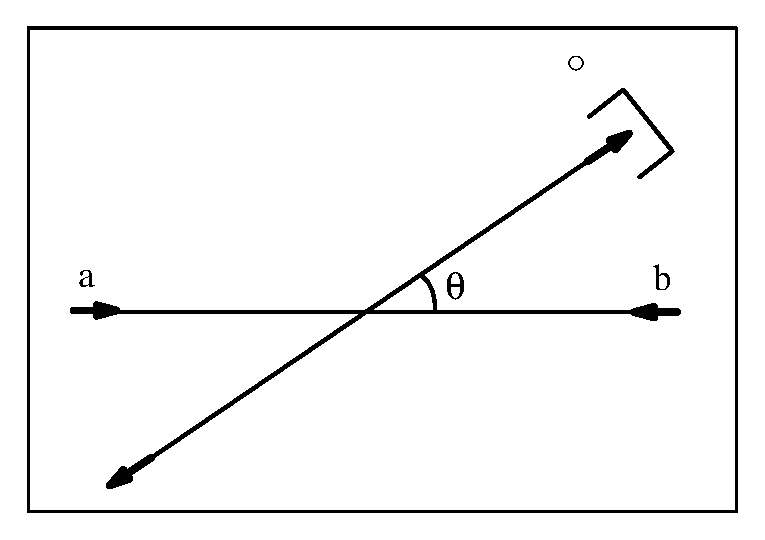
\includegraphics[clip,height=40mm,width=60mm]{1997phy4-1.eps}
\end{center}

\begin{subquestions}
\SubQuestion
aとbが異種粒子の時の散乱振幅を$f(\theta)$として、aとbが以下の場合について、それぞれの微分散乱断面積$\frac{d\sigma}{d\Omega}$を書き下せ。

\begin{subsubquestions}
\SubSubQuestion
aとbとが異種粒子、
\SubSubQuestion
aとbとが同種粒子でスピン0のボゾン、
\SubSubQuestion
aとbとが同種粒子でスピン$\frac{1}{2}$のフェルミオン。
\end{subsubquestions}

\SubQuestion
$_{\ 6}^{12}{\rm{C}}$(スピン0)と$^{13}_{\ 6}{\rm{C}}$(スピン$\frac{1}{2}$)をそれぞれ加速イオンビームまたは標的として、$^{12}{\rm{C}}+^{12}{\rm{C}}, ^{12}{\rm{C}}+^{13}{\rm{C}},^{13}{\rm{C}}+^{13}{\rm{C}}$の3つの組み合わせについて散乱実験を行った。加速器で10 {\Unit{MeV}}にまでイオンビームを加速したときの実験結果を下図に示した。重心系での角度で表示してある。但し、下図の縦軸・$\Deriver{\sigma}{\Omega}$は微分散乱断面積、下図の横軸・$\theta$は散乱角(重心系)[度]を表す。
\begin{center}
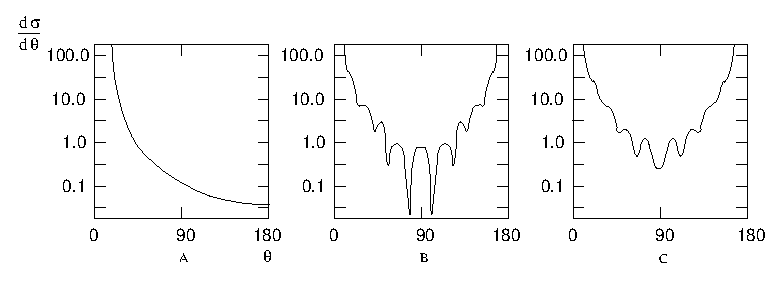
\includegraphics[clip,height=40mm,width=130mm]{1997phy4-2.eps}
\end{center}



\begin{subsubquestions}
\SubSubQuestion
aとbがともに$^{12}{\rm{C}}$と$^{12}{\rm{C}}$の時のドブロイ波長と重心系での運動エネルギー$T$を求めよ。
\SubSubQuestion
$^{12}{\rm{C}}$原子核の半径を$R$として、二つの原子核$^{12}{\rm{C}}$と$^{12}{\rm{C}}$がちょうど接触している状態の距離$2R$の位置でのクーロンポテンシャルによるエネルギー$V_C$を求め、$V_C>T$を確かめよ。このことから、散乱過程がこの入射エネルギー(10 {\Unit{MeV}})では主としてクーロン力によるものであることがわかる。
\SubSubQuestion
実験結果A,B,Cは、それぞれaとbが$^{12}{\rm{C}}$と$^{13}{\rm{C}}$のどの様な組合わせであるかを推論し、その理由を簡潔に述べよ。
\end{subsubquestions}

\SubSubQuestion
10{\Unit{MeV}}のビームエネルギーにおいても非常に小さな確率ではあるが、原子核反応
\[ ^{12}{\rm{C}}+^{12}{\rm{C}}\rightarrow ^{23}{\rm{Na}}^{*}+p \]
も起こる。ここで$^{23}{\rm{Na}}^*$は440 keVの励起準位を表し、平均寿命$1.1\times 10^{-12}$秒で$\gamma$線を放出して基底準位へおちる。
\begin{subsubquestions}
\SubSubQuestion
$\gamma$線の波長を求めよ。
\SubSubQuestion
励起準位の自然幅を求めよ。
\SubSubQuestion
なぜ非常に小さな確率でしか核反応は起きないのか。
\SubSubQuestion
$^{23}{\rm{Na}}^*$の最大速度$v$を求めよ。但し、簡単のために反応の${\rm{Q}}$値を0とする。
\[ [ {\rm{Q}}=2M_{^{12}{\rm{C}}}-(M_{^{23}{\rm{Na}}^*}+M_p)=0 ] \]
\SubSubQuestion
放出される$\gamma$線を、入射ビームの進行方向に置かれた$\gamma$線検出器で観測した。測定される$\gamma$線の最大ならびに最小エネルギーはいくらか。但し、生成された$^{23}{\rm{Na}}^*$イオンは、$10^{-12}$秒程度の時間で減速され標的中に止まるものとする。放出された$\gamma$線と標的物質との相互作用も無視する。
\SubSubQuestion
$\gamma$線と物質のとの相互作用にはどのようなものがあるか。
\SubSubQuestion
$\gamma$線の検出にNaI検出器を使い、440 keVの$\gamma$線を測定した。期待されるスペクトルの形を定性的に示し、どの様な相互作用が主に関与しているかをスペクトルの各部に記入せよ。
\end{subsubquestions}
\end{subquestions}
\end{question}
\begin{answer}{専攻 問題4}{}

\begin{subanswers}
\SubAnswer
\begin{subsubanswers}
\SubSubAnswer
aとbが異種粒子の時は、各々の入射波が干渉しあうことはないので
\[
\frac{d\sigma}{d\Omega}=|f(\theta)|^2
\]

\SubSubAnswer
aとbが同種粒子でスピン 0のボゾンの時、空間部分に対称性を持たせるために、
\begin{eqnarray*}
\frac{d\sigma}{d\Omega}&=&|f(\theta)+f(\pi-\theta)|^2\\
                       &=&|f(\theta)|^2+|f(\pi-\theta)|^2+2{\rm{Re}}[f(\theta)f(\pi-\theta)^{*}]
\end{eqnarray*}
となり、$|f(\theta)|$と$|f(\pi-\theta)|$が同時に観測され、かつ干渉を起こすことが分かる。

\SubSubAnswer
スピン1/2の2粒子は、合成スピン 0(1重項)の時はスピン部分が粒子の入れ替えに対して反対称であるので空間部分が対称、
合成スピン 1(3重項)の時はスピン部分が対称なので空間部分が反対称となることから、スピンを観測しないときの断面積は
\begin{eqnarray*}
\frac{d\sigma}{d\Omega}&=&\frac{1}{4}|f(\theta)+f(\pi-\theta)|^2+\frac{3}{4}|f(\theta)-f(\pi-\theta)|^2\\
                       &=&|f(\theta)|^2+|f(\pi-\theta)|^2-{\rm{Re}}[f(\theta)f(\pi-\theta)^{*}]
\end{eqnarray*}
となり、この場合も干渉を起こすことが分かる。

\end{subsubanswers}

\SubAnswer

\begin{subsubanswers}
\SubSubAnswer

実験室系で運動エネルギー$E_{L}$(速度$v_A$)の粒子a(質量$m_A$)が静止している粒子b(質量$m_B$)に衝突する過程
を重心系で見ると、重心速度$V=\frac{m_A v_A}{m_A+m_B}$(粒子aの進行方向を正とする)に対して粒子aは速度$v_A-V$、
粒子bは速度$V$で運動していることになるので、重心系での運動エネルギーは
\[
E_C=\frac{1}{2}m_A (v_A-V)^2+\frac{1}{2}m_B V^2=\frac{m_B}{m_A+m_B}E_L
\]
と表せる。今、$m_A=m_B=m_{^{12}{\rm{C}}}$、$E_L=10${\Unit{[MeV]}}であるので、重心系での運動エネルギーは$T=E_{\rm{C}}=\frac{1}{2}E_L=5${\Unit{[MeV]}}と
なる。

また、入射してくる$^{12}${\rm{C}}のドブロイ波長は非相対論的には以下の様に計算できる。
\[
\lambda=\frac{h}{p}=\frac{2\pi(\hbar c)}{\sqrt{2(M_{^{12}{\rm{C}}}c^2) E_L}}=\frac{2\pi\times 200{\Unit{[MeV]}}\cdot {\Unit{[fm]}}}{\sqrt{2\times 12000\times 10}{\Unit{[MeV]}}}
=2.56{\Unit{[fm]}}
\]
この結果は、原子核(1〜10{\Unit{[fm]}})の構造を調べるのに適していると言える。

\SubSubAnswer

電荷$+6e$の2つの原子核の中心が$2R$だけ離れた位置にあるとき、クーロン相互作用によるポテンシャルは
\[
V_{coulomb}=\frac{1}{4\pi\varepsilon_0}\frac{36e^2}{2R}=\frac{e^2}{4\pi\varepsilon_0 \hbar c}\frac{18\hbar c}{R}
\]
で与えられる。ここで、$R=1.2\times 12^{1/3}\simeq2.8${\Unit{[fm]}}、$\hbar c=200${\Unit{[MeV]}}$\cdot${\Unit{[fm]}}、
$\frac{e^2}{4\pi\varepsilon_0 \hbar c}=\frac{1}{137}$を用いて計算すると\fbox{$V_{coulomb}\simeq 9.4${\Unit{[MeV]}}}となる。
従って、$V_{coulomb}> T$が確かめられ、Rutherford散乱が中心の微分断面積が得られることが分かる。


\SubSubAnswer

{\bf 実験結果A:}\\
$\theta=90$度における微分断面積の対称性がないことから、干渉効果は見られず散乱後の2粒子は区別できるものである。
従って、$^{12}${\rm{C}}と$^{13}${\rm{C}}の弾性散乱の微分断面積であることが分かる。
\\
{\bf 実験結果B:}\\
重心系での散乱角が90度の時、微分断面積が極大となっている。これは、干渉項がプラスで効いているので、
ボゾン同士の散乱である。従って、$^{12}${\rm{C}}と$^{12}${\rm{C}}の弾性散乱。
\\
{\bf 実験結果C:}\\
重心系での散乱角が90度の時、微分断面積が極小となっている。これは、干渉項がマイナスで効いているので、
フェルミオン同士の散乱である。従って、$^{13}${\rm{C}}と$^{13}${\rm{C}}の弾性散乱。

[補足]\\
{\bf{1.(ii),(iii)}}を用いて、散乱角が90度の時の微分断面積を求めると、
\begin{eqnarray*}
\Bigl(\frac{d\sigma}{d\Omega}\Bigr)_{Boson}\Bigl(\theta=\frac{\pi}{2}\Bigr)&=&4\left|f\Bigl(\frac{\pi}{2}\Bigr)\right|^2 \\
\Bigl(\frac{d\sigma}{d\Omega}\Bigr)_{Fermion}\Bigl(\theta=\frac{\pi}{2}\Bigr)&=&\left|f\Bigl(\frac{\pi}{2}\Bigr)\right|^2 
\end{eqnarray*}
と計算できる。ここで、与えられたグラフを見ると、$\theta=90$度の微分断面積の値がBでは0.8、{\rm{C}}では0.2程度なので
上の考察が正しいことが確認できる。
\end{subsubanswers}

\SubAnswer

\begin{subsubanswers}

\SubSubAnswer
$400{\Unit{keV}}$の励起状態から、基底状態へ落ちるときに放出されるγ線の波長は、
\[
\lambda=\frac{hc}{E}=\frac{2\pi\hbar c}{E}=\frac{2\pi  \times 200 {\Unit{[MeV]}} \cdot {\Unit{[fm]}}}{400 \times 10^{-3}{[\Unit{MeV}]}}=2.9\times 10^{-12} [{\Unit{m}}]
\]

\SubSubAnswer
自然幅$\Gamma$、平均寿命$\tau$の間には不確定性関係$\Gamma\cdot\tau=\hbar$が成り立っていることより、
\[
\Gamma=\frac{\hbar c}{\tau c}=\frac{200{\Unit{[MeV]}}\cdot {\Unit{[fm]}}}{1.1\times 10^{-12}\times 3\times 10^{23}{\Unit{[fm]}}}\simeq 6\times 10^{-4}{\Unit{[eV]}}
\]

\SubSubAnswer
核反応に関与する力は短距離力である強い相互作用であるため、2つの原子核が十分に近づかなければ反応は起こらない。今回の実験では、入射エネルギーが十分でないために、クーロン斥力に打ち勝って接近しにくいためであると考えられる。


\SubSubAnswer

\parbox[t]{100mm}{反応のQ値が$0$であるという仮定より、古典力学の弾性衝突の問題として扱える。図のような衝突過程を考えると
エネルギー保存則、運動エネルギー保存則より、
\begin{eqnarray}
m_{{\rm{C}}}v_{0}&=&m_{{\rm{Na}}}v\cos\theta+m_p v'\cos\phi \eqname{3-3-0}   \\
0&=&m_{{\rm{Na}}}v\sin\theta-m_p v'\sin\phi    \eqname{3-3-1}   \\
\frac{1}{2}m_{{\rm{C}}}v_{0}^{2}&=&\frac{1}{2}m_{{\rm{Na}}}v^2+\frac{1}{2}m_{p}v^{\prime 2} \eqname{3-3-2}
\end{eqnarray}}
\parbox[t]{60mm}{\vspace*{-3mm}
\begin{center}
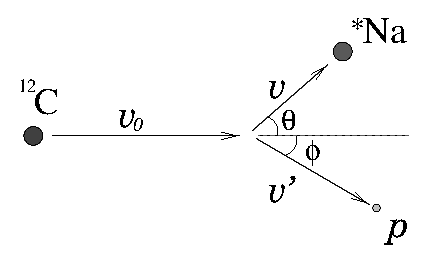
\includegraphics[clip,height=36mm,width=50mm]{1997phy4-4.eps}
\end{center}
}

この3式より観測にかからない量$v'$と$\phi$を消去する。\eqhref{3-3-0},\eqhref{3-3-1}より$\phi$を消去すると
\begin{equation}
(m_{\rm{C}} v_0-m_{{\rm{Na}}}v\cos\theta)^2+(m_{{\rm{Na}}}v\sin\theta)^2=(m_p v')^2 \eqname{3-3-3}
\end{equation}
\eqhref{3-3-2},\eqhref{3-3-3}より、$v'$を消去して、$v$の方程式にすると、
\[
m_{{\rm{Na}}}(m_{{\rm{Na}}}+m_{{\rm{p}}})v^2-2(m_C m_{{\rm{Na}}}v_0 \cos\theta)v+m_{\rm{C}}(m_{\rm{C}}-m_p)v_0^2=0
\]

上式の解は
\[
v=\frac{m_{\rm{C}} m_{{\rm{Na}}}v_0\cos\theta\pm\sqrt{(m_{\rm{C}} m_{{\rm{Na}}}v_0 \cos\theta)^2-m_{\rm{C}} m_{{\rm{Na}}}(m_{{\rm{Na}}}+m_{p})(m_{\rm{C}}-m_p)v_0^2}}{m_{{\rm{Na}}}(m_{{\rm{Na}}}+m_p)}
\]
これより、$v$の最大値は$\cos\theta=1$、複号プラスの時で
\begin{eqnarray*}
v_{max}&=&\frac{m_{\rm{C}} m_{{\rm{Na}}}+\sqrt{(m_{\rm{C}} m_{{\rm{Na}}})^2-m_{\rm{C}} m_{{\rm{Na}}}(m_{{\rm{Na}}}+m_p)(m_{\rm{C}}-m_p)}}{m_{{\rm{Na}}}(m_{{\rm{Na}}}+m_p)}v_0\\
       &=&\frac{m_{\rm{C}}}{m_{{\rm{Na}}}+m_p}\Bigl[1+\sqrt{1-(1+\frac{m_p}{m_{{\rm{Na}}}})(1-\frac{m_p}{m_{\rm{C}}})}\Bigr] v_0
\end{eqnarray*}
ここで、$v_0=\sqrt{\frac{2\times 10{\Unit{[MeV]}}}{12\times 1000{\Unit{[MeV]}}}}c=0.04c$($c$:光速)より、
\[
v_{max}=\frac{12}{23+1}\Bigl[1+\sqrt{1-(1+\frac{1}{23})(1-\frac{1}{12})}\Bigr]v_0=0.024c
\]

\SubSubAnswer
$^{23}${\rm{Na}}$^{*}$が標的中で減速される際に失うエネルギーは、放出される$\gamma$線のエネルギーには変化をもたらさない。
従って、$\gamma$線のエネルギーを変化させるものは主に$^{23}${\rm{Na}}$^{*}$のもつ速度による放出$\gamma$線のドップラー効果
である。光のドップラー効果は相対論を用いる必要がある。\\

{\bf γ線のエネルギーが最大:}\\
入射粒子と同じ向きに運動している$^{23}${\rm{Na}}$^{*}$が生成されると同時に$\gamma$線を放射するときで、
\[
E'=h\nu'=h\sqrt{\frac{1+\beta}{1-\beta}}\nu=\sqrt{\frac{1+\beta}{1-\beta}}E=451{\Unit{[keV]}}
\]
非相対論的に$\ds{\sqrt{\frac{1+\beta}{1-\beta}}}=1+\beta+{\rm{O}}(\beta^2)$として、2次以上の項を無視して計算しても同じ結果になる。
\bigskip

{\bf γ線のエネルギーが最小:}\\
核反応によって生じた$^{23}${\rm{Na}}$^{*}$が標的の中で完全に静止した後に$\gamma$線を放射するときで、
\[
E'=E=440{\Unit{[keV]}}
\]
エネルギー保存則から、入射方向と反対方向に$v_{max}$で$^{23}{\rm{Na}}^{*}$が出ていくことは有り得ないことに注意。

\SubSubAnswer
γ線と物質との相互作用は主に以下に3つがある。\\
{\bf 光電効果\\}
γ線が原子に吸収されて、主としてK殻の電子が運動エネルギー$E=h\nu-(仕事関数)$で飛び出してくる現象。
低エネルギーのγ線領域で支配的。
\\
{\bf コンプトン散乱\\}
原子中の電子の束縛エネルギーが無視できるほど入射光子のエネルギーが大きくなると、光子と自由電子の衝突という
描像が成り立ち、自由電子による光子の散乱が生じる。これを、コンプトン散乱という。
\\
{\bf 電子対生成\\}
光子のエネルギーが非常に大きくなると、物質中の電磁場とγ線の相互作用により、電子と陽電子の対が生成される。この時、
必要な光子のエネルギーは、Diracの海に沈んでいる電子をたたき出すエネルギーなので、$2m_e c^2=1.02${\Unit{[MeV]}}となる。

\SubAnswer
NaIシンチレーションカウンタのエネルギースペクトルは下図のようになる。光電吸収ピークのエネルギーが$440[{\Unit{keV}}]$に一致している。
\begin{center}
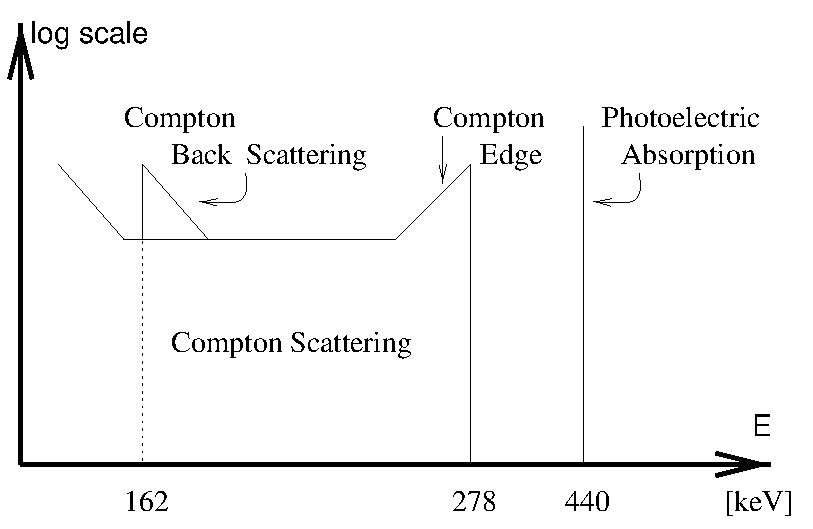
\includegraphics[clip,width=102mm,height=61mm]{1997phy4-5.eps}
\end{center}

\end{subsubanswers}
\end{subanswers}
\end{answer}


\end{document}
